\documentclass[11pt,a4paper]{article}

\usepackage[a4paper,margin=1in]{geometry}
\usepackage[T1]{fontenc}
\usepackage[utf8]{inputenc}
\usepackage{lmodern}

\usepackage{microtype}
\usepackage{graphicx}
\usepackage{booktabs}
\usepackage{amsmath,amssymb}
\usepackage{hyperref}
\usepackage{pdfpages} % for including pre-rendered PDFs if needed

\hypersetup{
  colorlinks=true,
  linkcolor=blue,
  urlcolor=blue,
  citecolor=blue
}

\title{Data Science in Medical Imaging\\Coursework Minor A2}
\author{Candidate: hb747}
\date{March 2026}

\begin{document}
\maketitle

\begin{abstract}
This report accompanies the submitted code and experiments for the three coursework modules: tomographic reconstruction, MRI denoising, and a written critical comparison of segmentation methods. Quantitative metrics are reported alongside representative visual outputs, and parameter settings are stated so results can be reproduced from a clean checkout.
\end{abstract}

\tableofcontents
\newpage

\section{Reproducibility notes}
\begin{itemize}
  \item Code lives in \texttt{med\_im/}. Experiments are run from \texttt{notebooks/} (and any scripts referenced there).
  \item Figures and tables used in this report should be generated by tracked code; each figure caption states which notebook/script produced it.
  \item Random seeds and key parameters (noise level, number of projections, angular range, filter settings) are stated next to results.
\end{itemize}

\section{Module 1: Tomographic reconstruction}

\subsection{Exercise 1.1: Reducing dose}
\subsubsection*{Setup}
The CT slice provided in the coursework was loaded from \texttt{data/CT\_exercise\_1.png} and converted to grayscale. The working image size was $512\times512$ pixels with intensity range approximately $[0, 10^{-3}]$.

\begin{figure}[p]
  \centering
  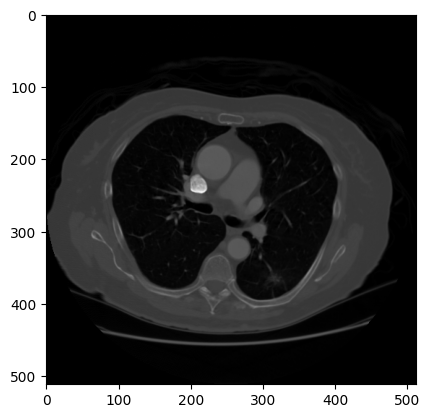
\includegraphics[width=0.7\linewidth]{development_notebook_files/development_notebook_3_1.png}
  \caption{Input CT image used for Module 1 (generated in \texttt{notebooks/development.ipynb}).}
\end{figure}

\subsubsection*{Noise simulation}
Noisy sinograms were simulated by combining Poisson noise on the transmitted intensity with additive Gaussian noise on top. The Gaussian component used $\mu = 0$ and $\sigma = 0.05$ while the Poisson component used three incident fluence settings $I_0 \in \{10^5, 10^3, 10^2\}$. Each condition was simulated at three projection counts $N_\theta \in \{360, 90, 20\}$.

\begin{figure}[p]
  \centering
  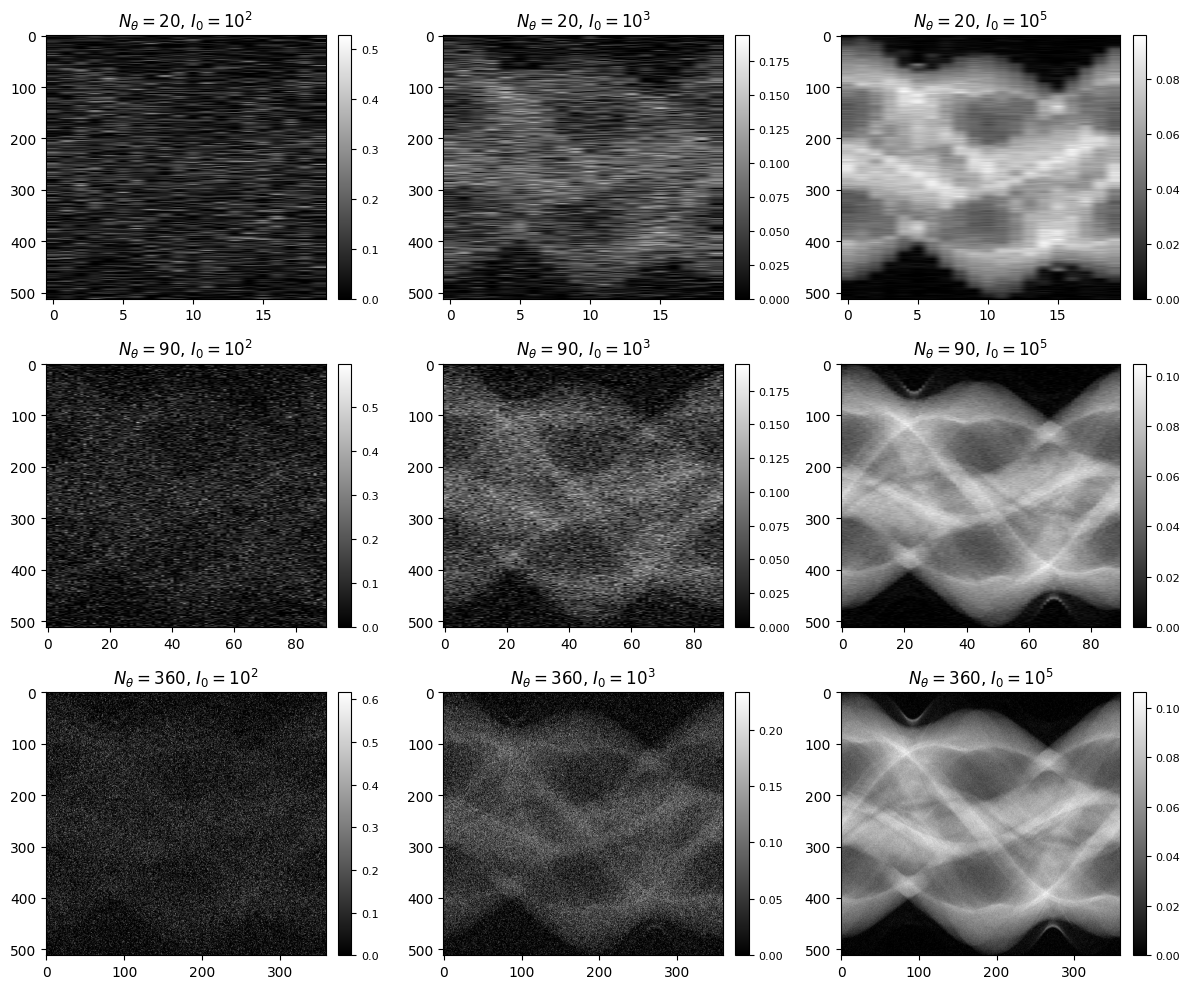
\includegraphics[width=\linewidth]{development_notebook_files/development_notebook_5_1.png}
  \caption{Noisy sinograms across projection count ($N_\theta$) and dose setting ($I_0$) (generated in \texttt{notebooks/development.ipynb}).}
\end{figure}

\subsubsection*{Reconstructions: FBP vs gradient descent (SIRT)}
Each noisy sinogram was reconstructed using filtered back-projection (FBP, ramp/Ram--Lak filter) and a simple gradient descent / SIRT-style update using repeated backprojection of the residual.

\begin{figure}[p]
  \centering
  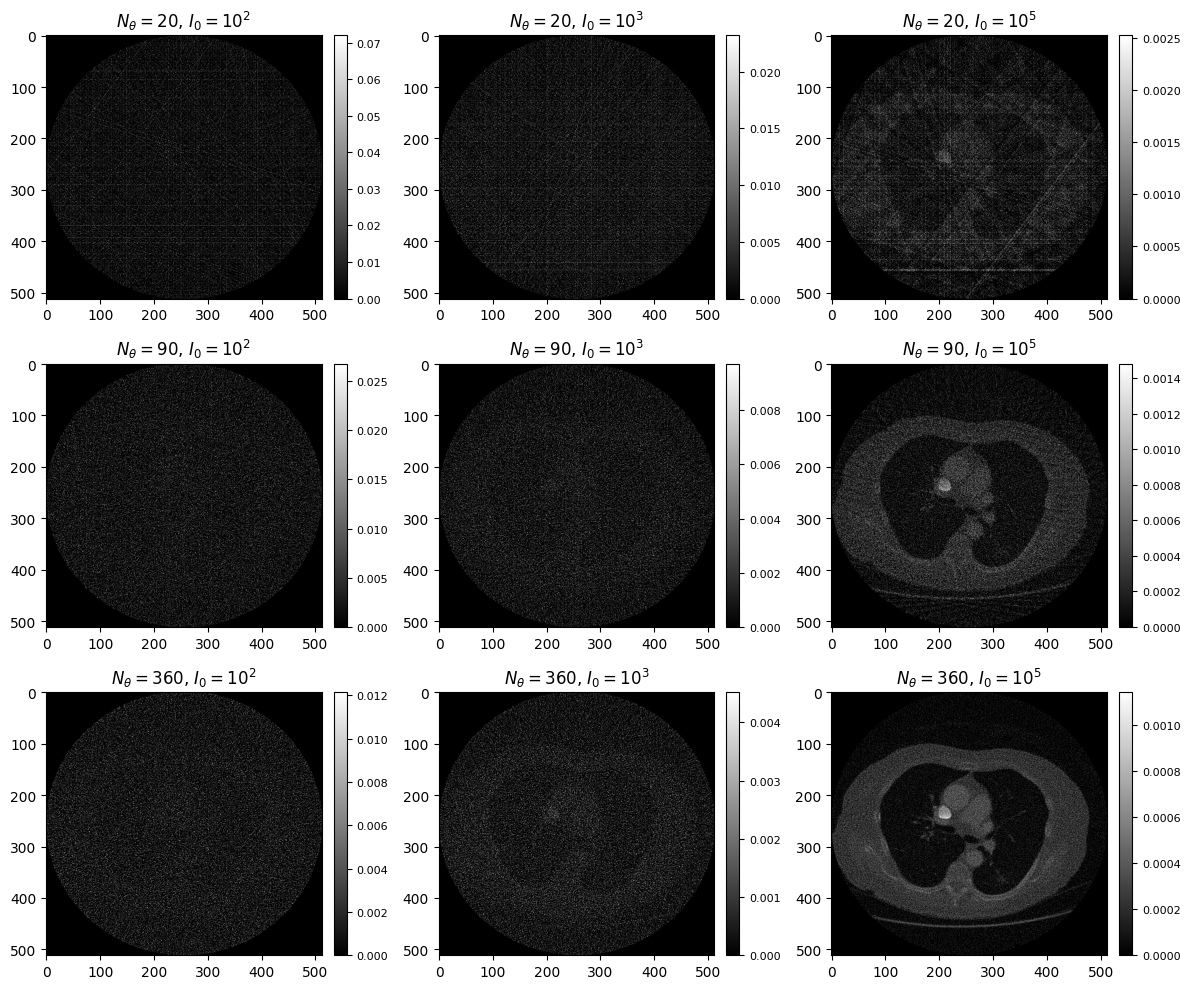
\includegraphics[width=\linewidth]{development_notebook_files/development_notebook_7_0.png}
  \caption{FBP reconstructions across $N_\theta$ and $I_0$ (generated in \texttt{notebooks/development.ipynb}).}
\end{figure}

\begin{figure}[p]
  \centering
  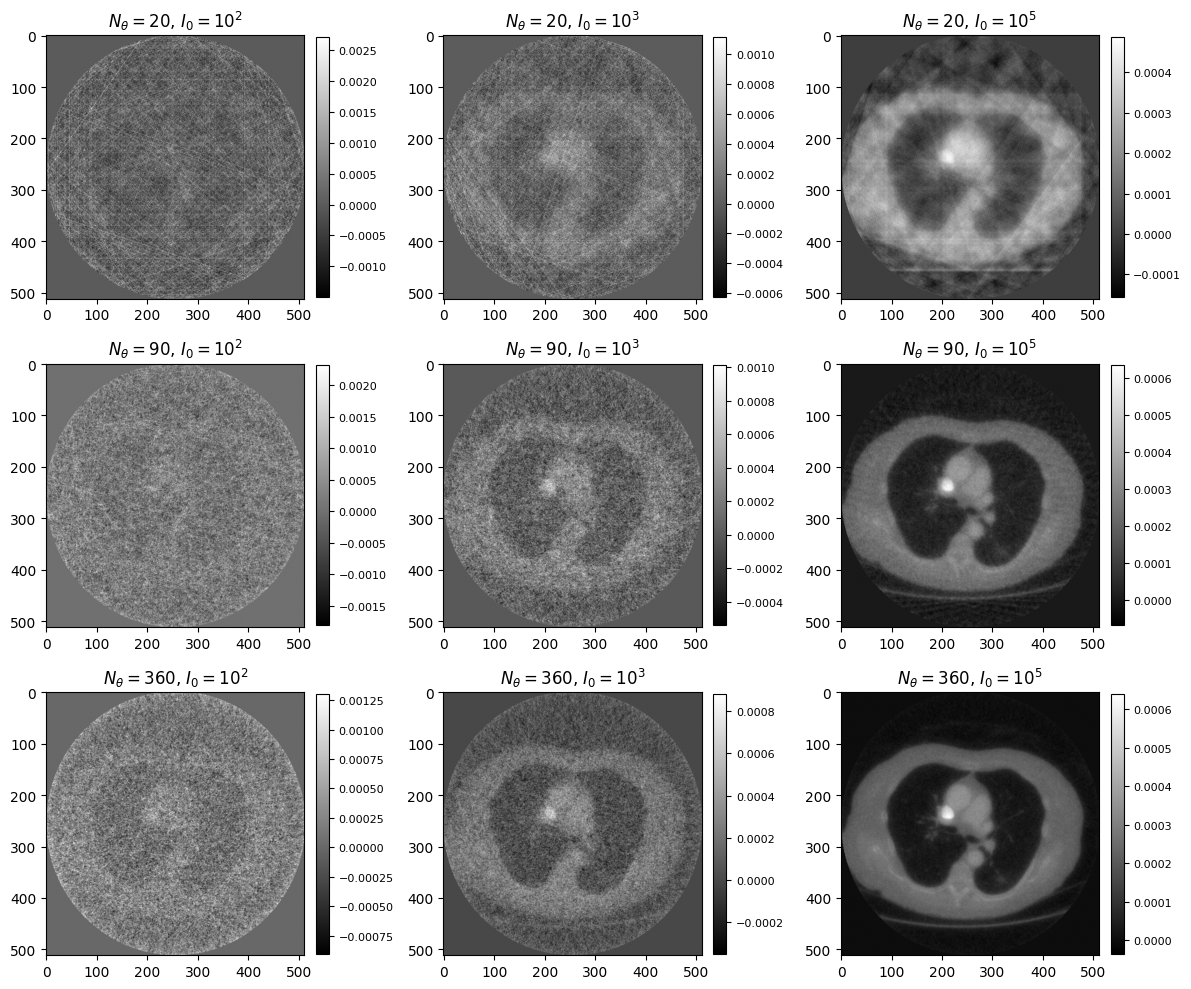
\includegraphics[width=\linewidth]{development_notebook_files/development_notebook_8_0.png}
  \caption{Gradient descent / SIRT reconstructions across $N_\theta$ and $I_0$ (generated in \texttt{notebooks/development.ipynb}).}
\end{figure}

\subsubsection*{Clinical interpretation}
Reducing $I_0$ (dose) and reducing the number of angles both degraded reconstruction quality; in the lowest dose / sparse-angle settings the reconstructions show more visible artefacts and loss of fine structure, which would plausibly make small lesions or subtle edges harder to detect. In practice there is a trade-off between radiation exposure, acquisition time, and diagnostic reliability, and iterative methods may partially compensate for reduced data but cannot fully recover missing information.

\subsubsection*{How to get better images}
Two straightforward ways to improve quality in these settings are to add explicit regularisation (for example, total variation or edge-preserving penalties) and to use more accurate statistical models for the noise (e.g. Poisson likelihood rather than a simple least-squares residual). A third option is to use learned priors or plug-and-play denoisers inside an iterative reconstruction loop, although this requires careful validation.

\subsection{Exercise 1.2: Limited angle tomography}
\subsubsection*{Setup and simulations}
The same dose and projection-count experiment from Exercise 1.1 was repeated using limited angular coverage. Three angular ranges were tested: $180^\circ$, $120^\circ$, and $40^\circ$.

\begin{figure}[p]
  \centering
  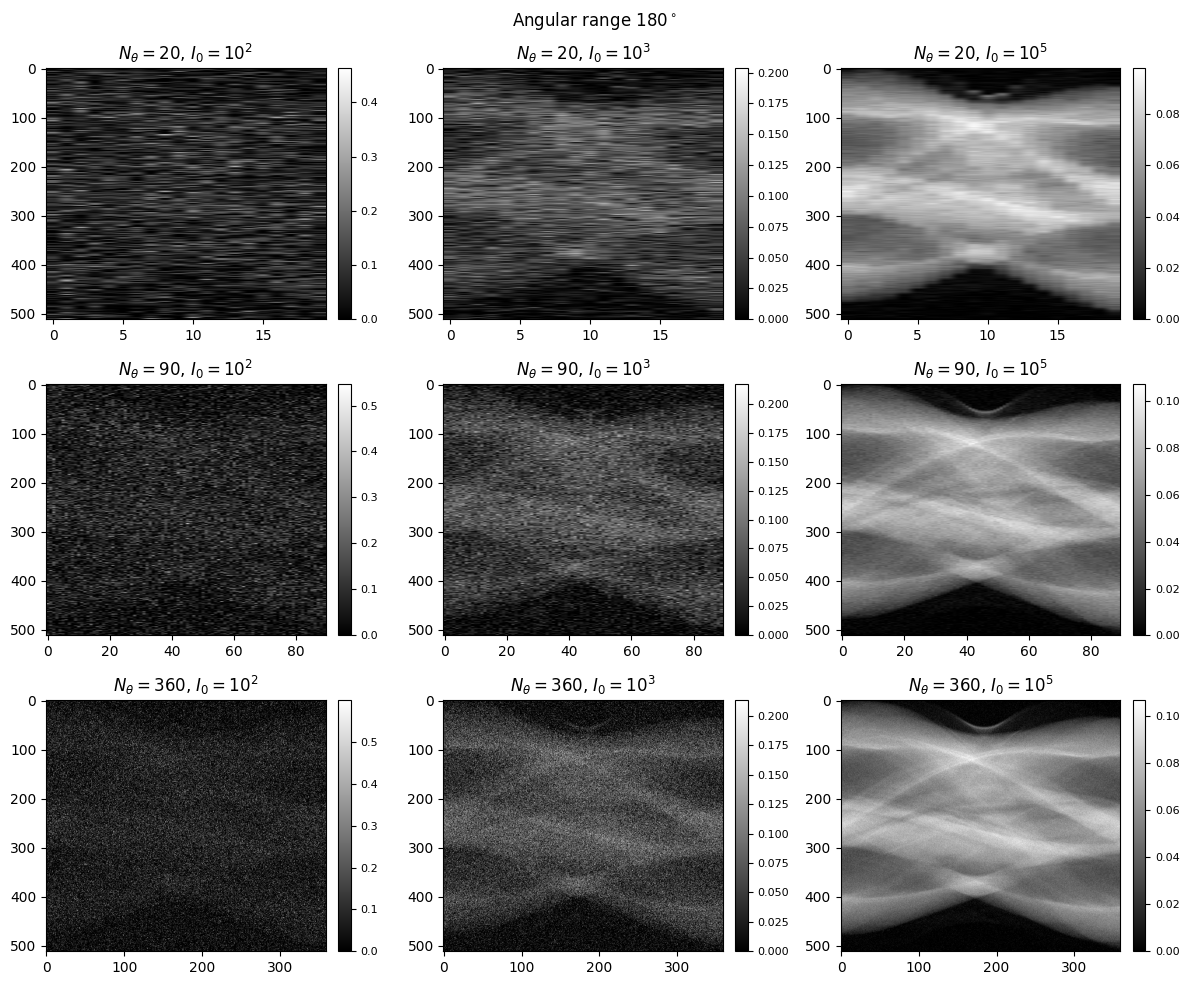
\includegraphics[width=\linewidth]{development_notebook_files/development_notebook_10_0.png}
  \caption{Noisy sinograms for angular range $180^\circ$ (generated in \texttt{notebooks/development.ipynb}).}
\end{figure}

\begin{figure}[p]
  \centering
  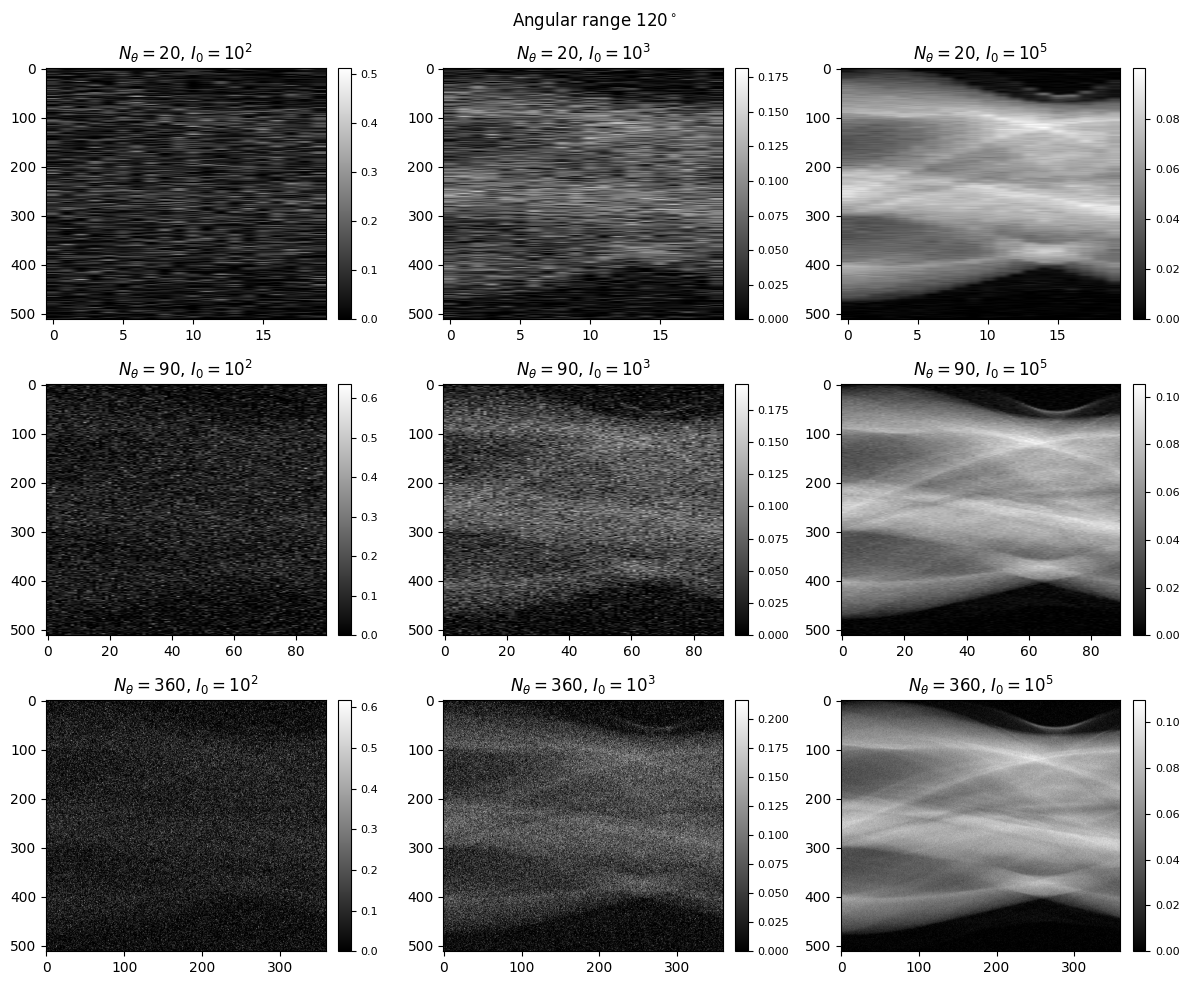
\includegraphics[width=\linewidth]{development_notebook_files/development_notebook_10_1.png}
  \caption{Noisy sinograms for angular range $120^\circ$ (generated in \texttt{notebooks/development.ipynb}).}
\end{figure}

\begin{figure}[p]
  \centering
  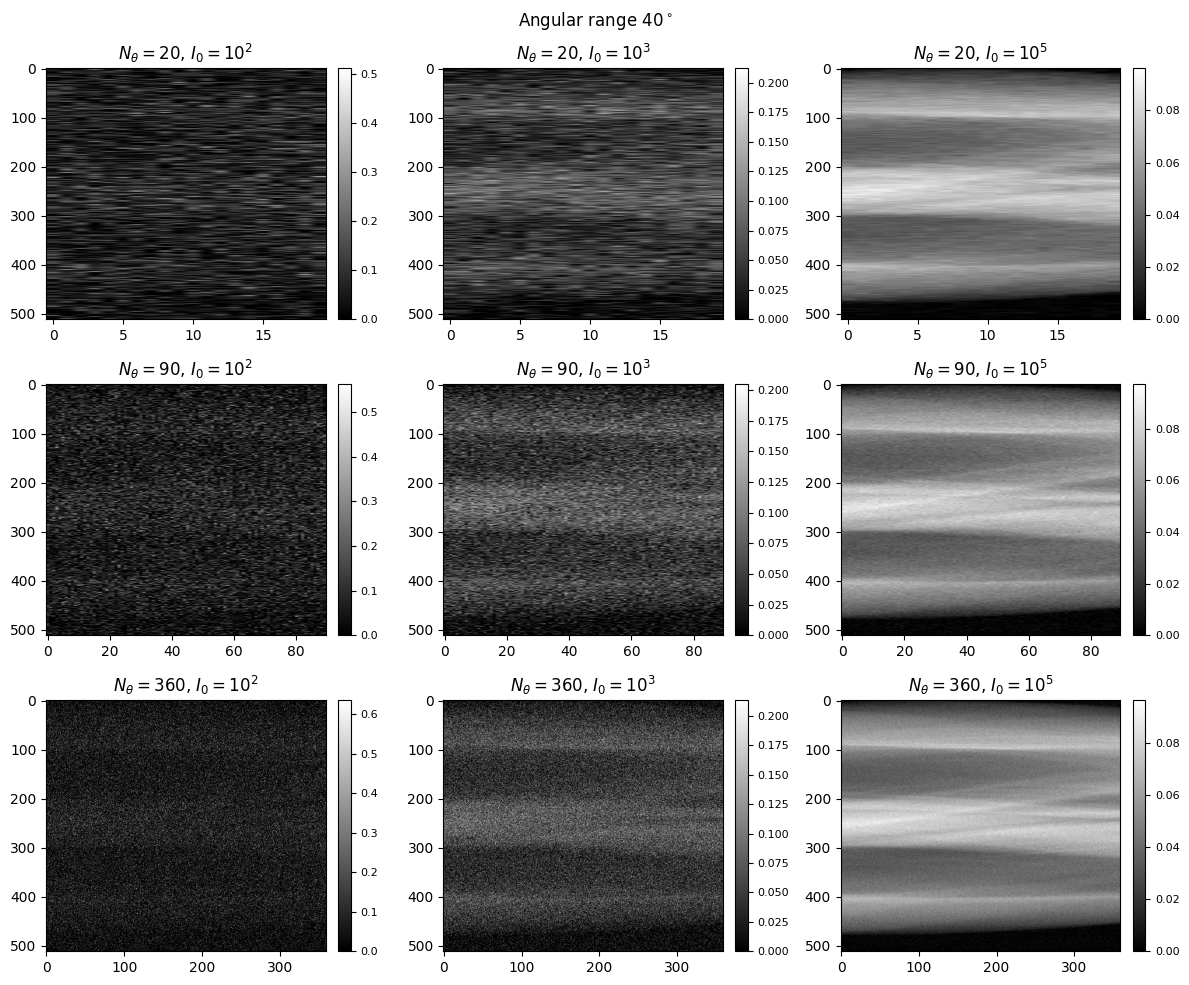
\includegraphics[width=\linewidth]{development_notebook_files/development_notebook_10_2.png}
  \caption{Noisy sinograms for angular range $40^\circ$ (generated in \texttt{notebooks/development.ipynb}).}
\end{figure}

\subsubsection*{Observed differences and explanation}
As the angular range shrinks, the reconstruction becomes increasingly anisotropic: some edges are recovered reasonably while others smear into streaks. This is consistent with the Fourier slice theorem intuition: limited angle sampling leaves regions of frequency space unmeasured (a ``missing wedge''), so features aligned with those missing frequencies are poorly constrained.

\begin{figure}[p]
  \centering
  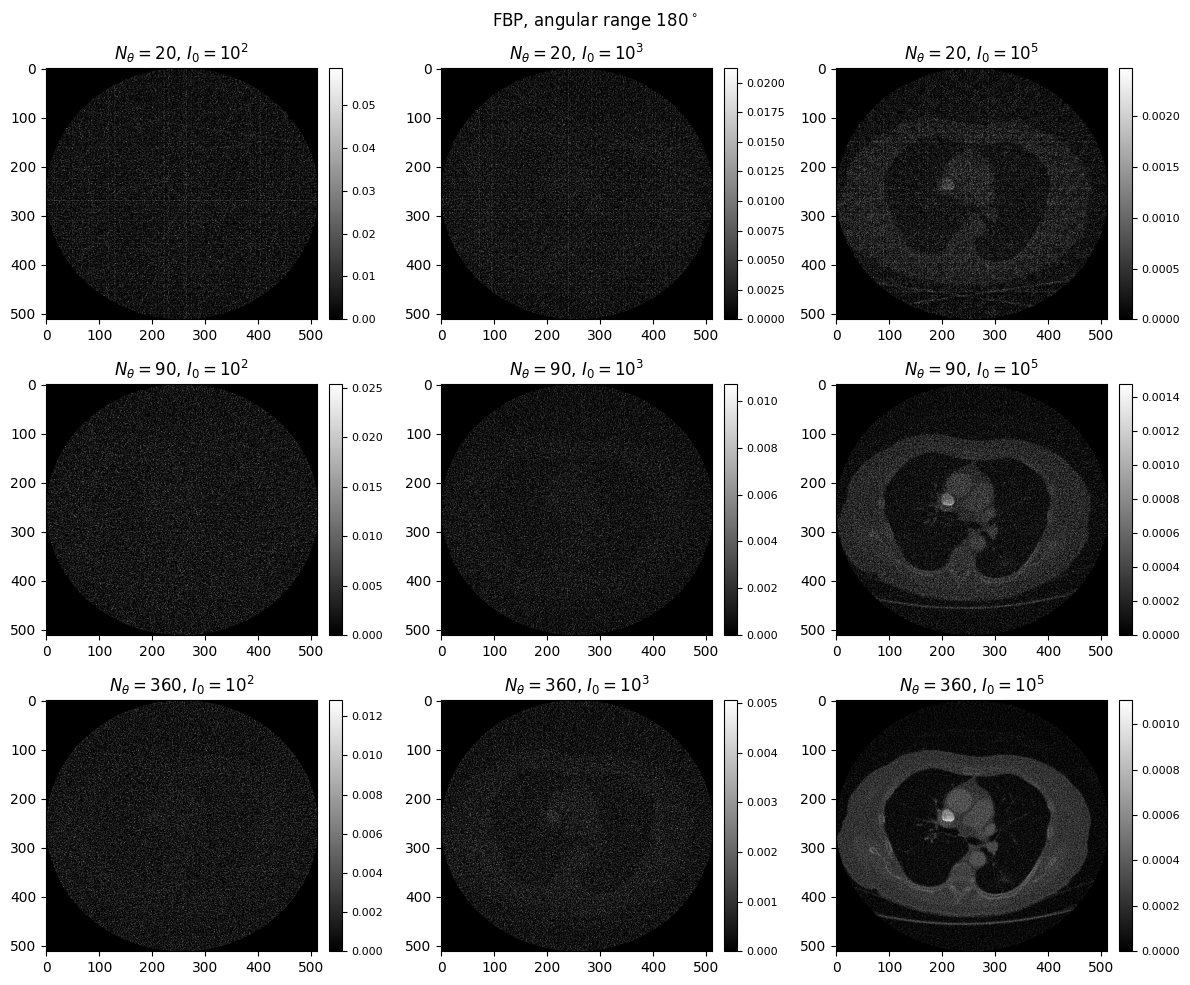
\includegraphics[width=\linewidth]{development_notebook_files/development_notebook_12_0.png}
  \caption{FBP reconstructions at $180^\circ$ angular range (generated in \texttt{notebooks/development.ipynb}).}
\end{figure}
\begin{figure}[p]
  \centering
  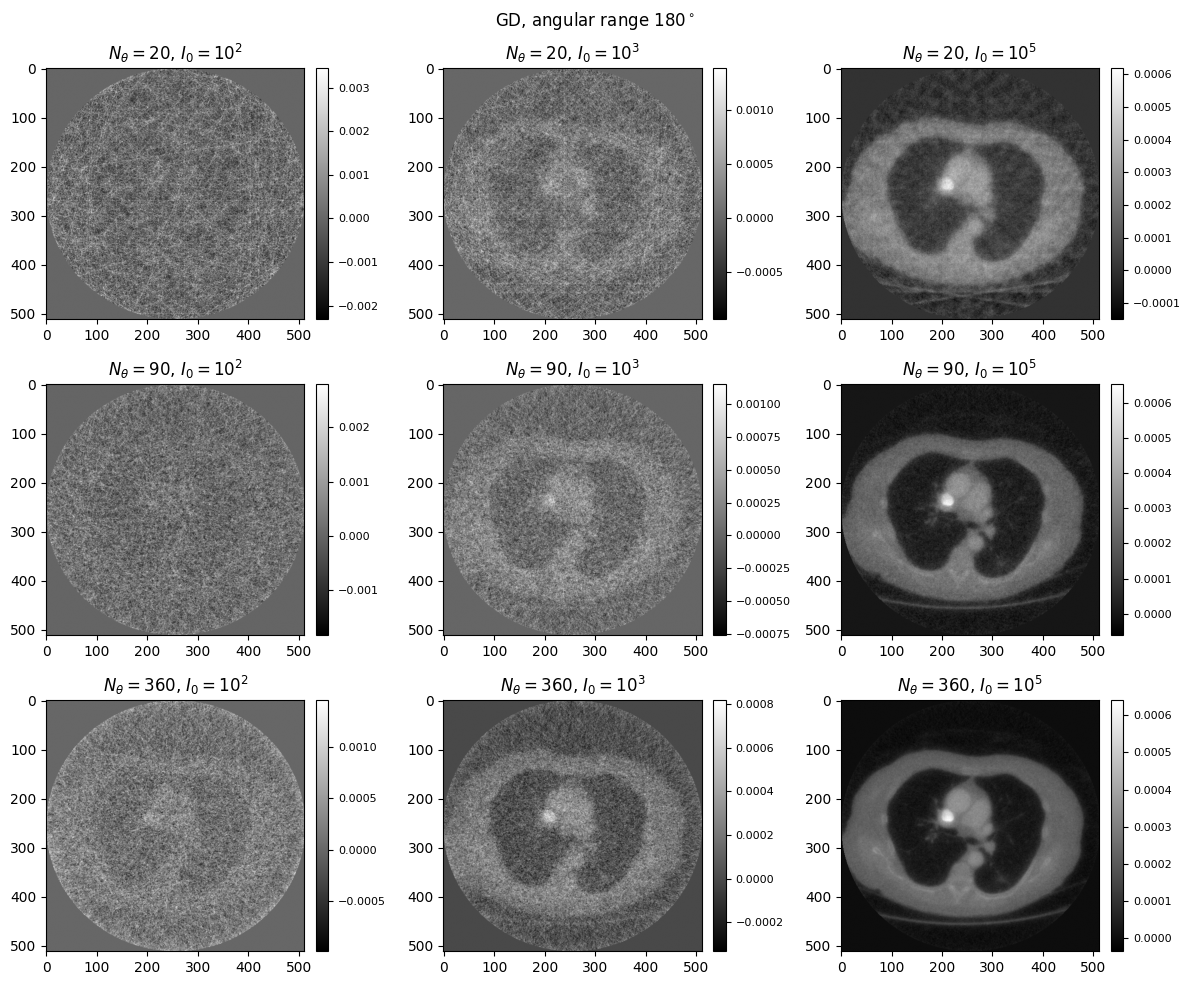
\includegraphics[width=\linewidth]{development_notebook_files/development_notebook_12_1.png}
  \caption{GD/SIRT reconstructions at $180^\circ$ angular range (generated in \texttt{notebooks/development.ipynb}).}
\end{figure}
\begin{figure}[p]
  \centering
  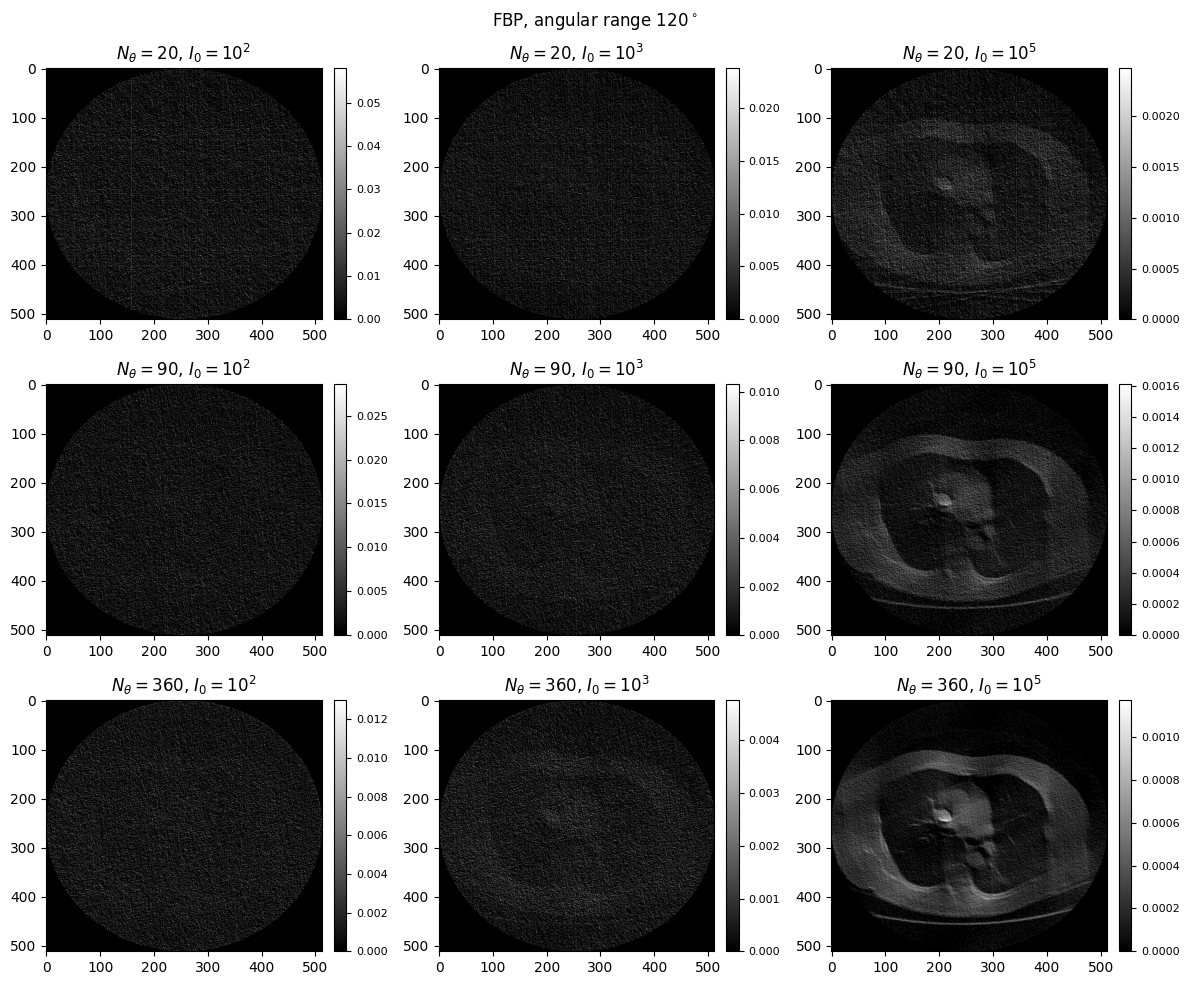
\includegraphics[width=\linewidth]{development_notebook_files/development_notebook_12_2.png}
  \caption{FBP reconstructions at $120^\circ$ angular range (generated in \texttt{notebooks/development.ipynb}).}
\end{figure}
\begin{figure}[p]
  \centering
  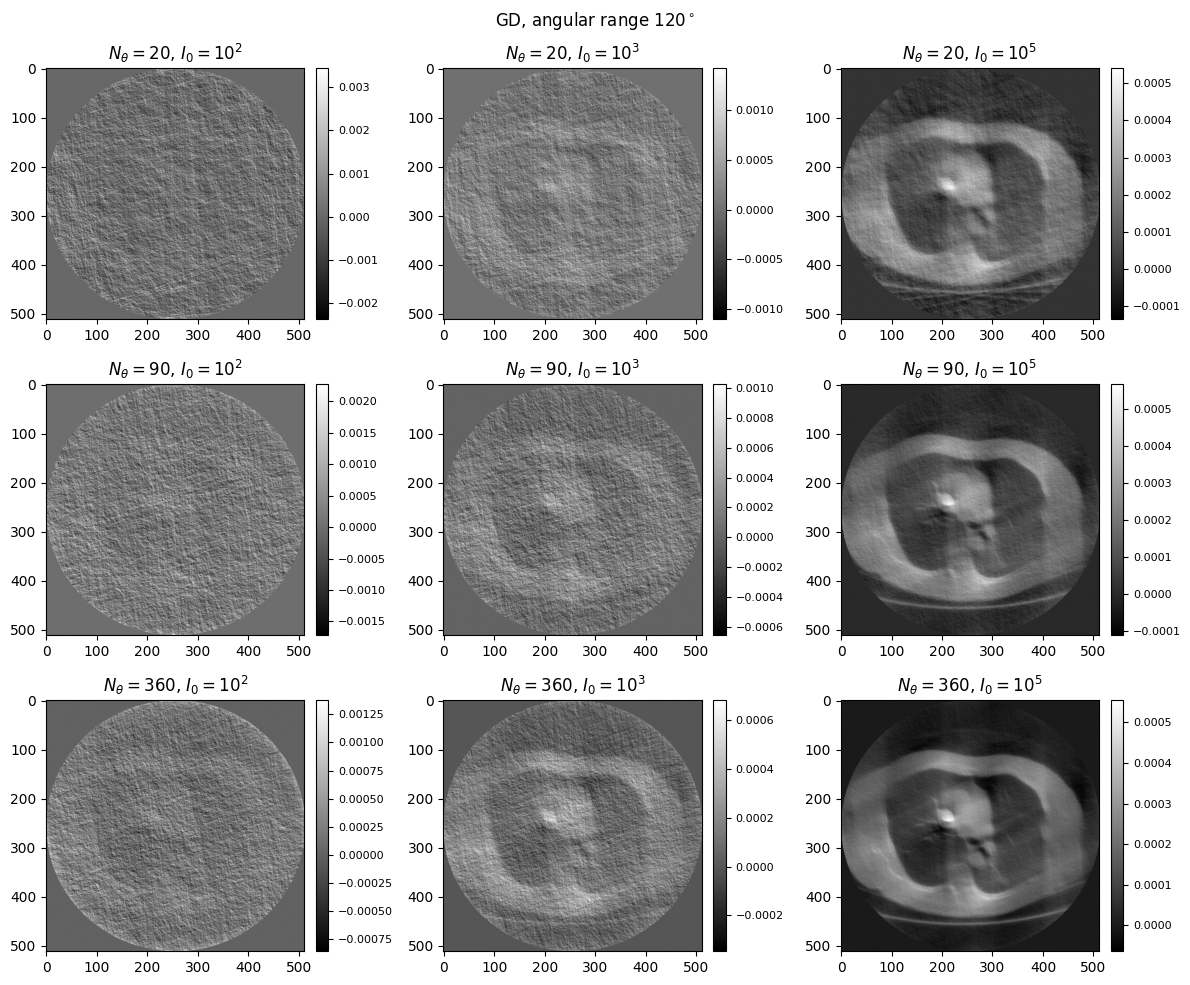
\includegraphics[width=\linewidth]{development_notebook_files/development_notebook_12_3.png}
  \caption{GD/SIRT reconstructions at $120^\circ$ angular range (generated in \texttt{notebooks/development.ipynb}).}
\end{figure}
\begin{figure}[p]
  \centering
  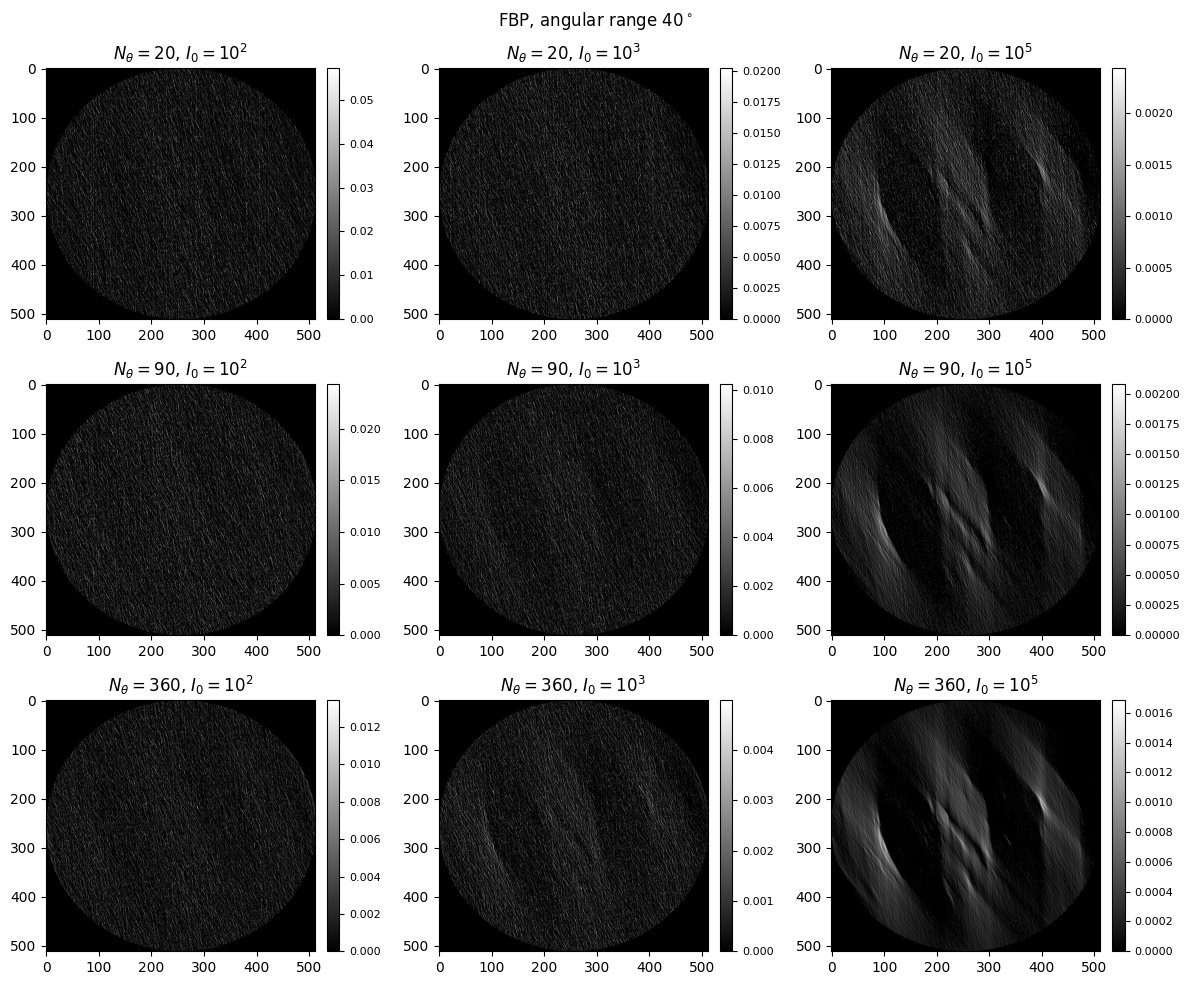
\includegraphics[width=\linewidth]{development_notebook_files/development_notebook_12_4.png}
  \caption{FBP reconstructions at $40^\circ$ angular range (generated in \texttt{notebooks/development.ipynb}).}
\end{figure}
\begin{figure}[p]
  \centering
  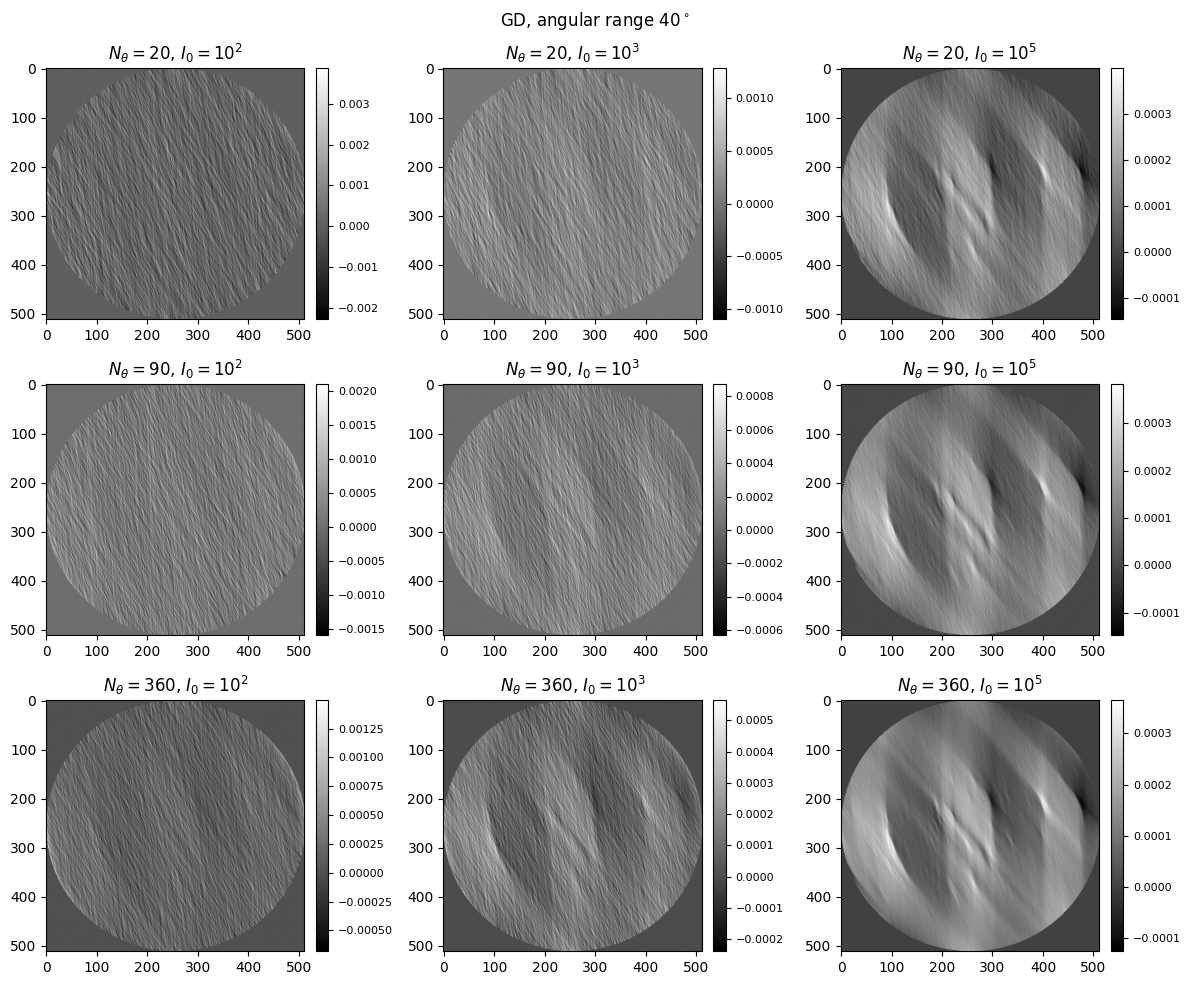
\includegraphics[width=\linewidth]{development_notebook_files/development_notebook_12_5.png}
  \caption{GD/SIRT reconstructions at $40^\circ$ angular range (generated in \texttt{notebooks/development.ipynb}).}
\end{figure}

\subsection{Exercise 1.3: Reconstruction}
\subsubsection*{Alternative FBP filters}
Two alternative filters tested here were:
\begin{itemize}
  \item Shepp--Logan: a ramp filter multiplied by a sinc window, which rolls off very high frequencies and can reduce noise while keeping edges fairly sharp.
  \item Cosine: a ramp filter multiplied by a cosine window, which suppresses high frequencies more strongly; this tends to look smoother but also more blurred.
\end{itemize}

\begin{figure}[p]
  \centering
  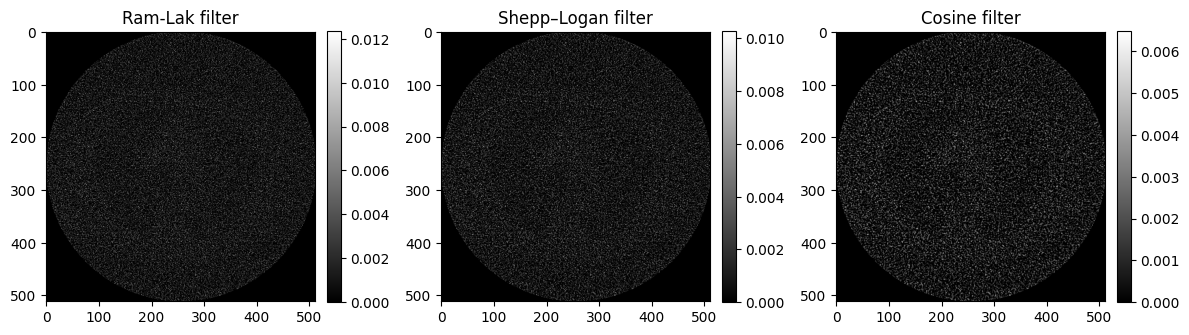
\includegraphics[width=\linewidth]{development_notebook_files/development_notebook_14_0.png}
  \caption{Filter comparison (Ram--Lak / Shepp--Logan / Cosine) on a low-dose example (generated in \texttt{notebooks/development.ipynb}).}
\end{figure}

\subsubsection*{OS-SART / ordered subsets vs SIRT}
Ordered subsets updates (OS-SART) were implemented by splitting projection angles into subsets and updating the image multiple times per iteration. In this small experiment OS-SART gives a similar qualitative reconstruction to full-batch SIRT but with different convergence behaviour depending on subset size and step size.

\begin{figure}[p]
  \centering
  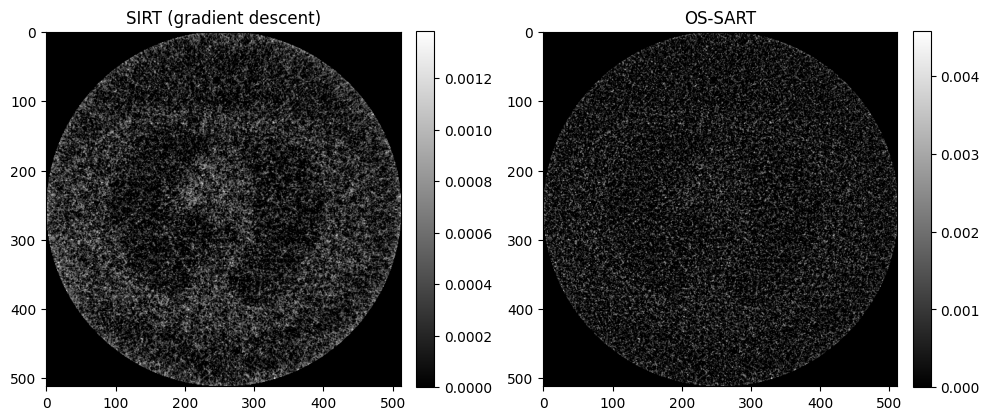
\includegraphics[width=\linewidth]{development_notebook_files/development_notebook_16_0.png}
  \caption{Comparison of SIRT (gradient descent) vs OS-SART for the same acquisition setting (generated in \texttt{notebooks/development.ipynb}).}
\end{figure}

\subsubsection*{PET vs CT iterative methods}
% TODO: Discuss why MLEM/OSEM is natural for Poisson emission data, while least-squares style updates are common in CT.

\section{Module 2: MRI image denoising}

\subsection{Exercise 2.1: Visualisation and identifying noise}
\subsubsection*{k-space and coil dimension}
The k-space data (\texttt{data/knee.npy}) was loaded as a 3D array with the coil dimension on axis 0 (six coils). Log-magnitude k-space was plotted for each coil.

\begin{figure}[p]
  \centering
  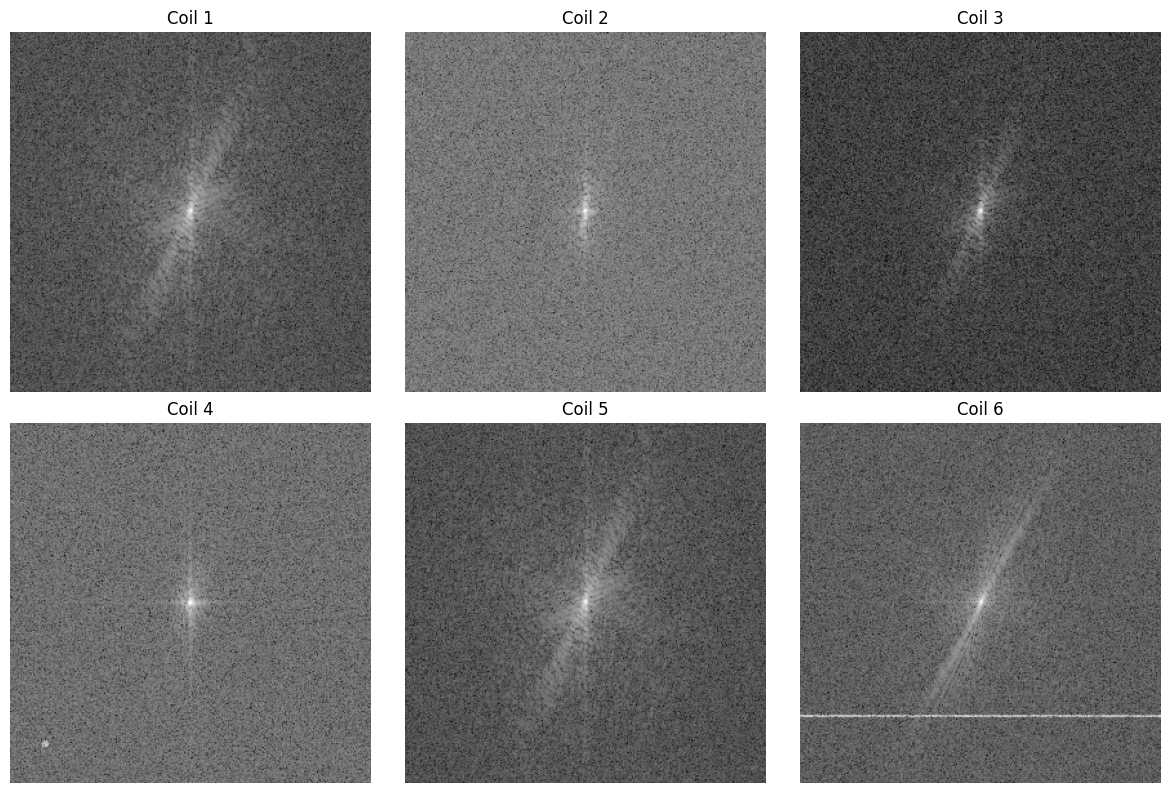
\includegraphics[width=\linewidth]{development_notebook_files/development_notebook_18_1.png}
  \caption{Log-magnitude k-space for each coil (generated in \texttt{notebooks/development.ipynb}).}
\end{figure}

\subsubsection*{Image-space magnitude and phase}
Each coil was transformed to image space using an inverse FFT. For one coil, both magnitude and phase images were visualised, then magnitude images were shown across all coils.

\begin{figure}[p]
  \centering
  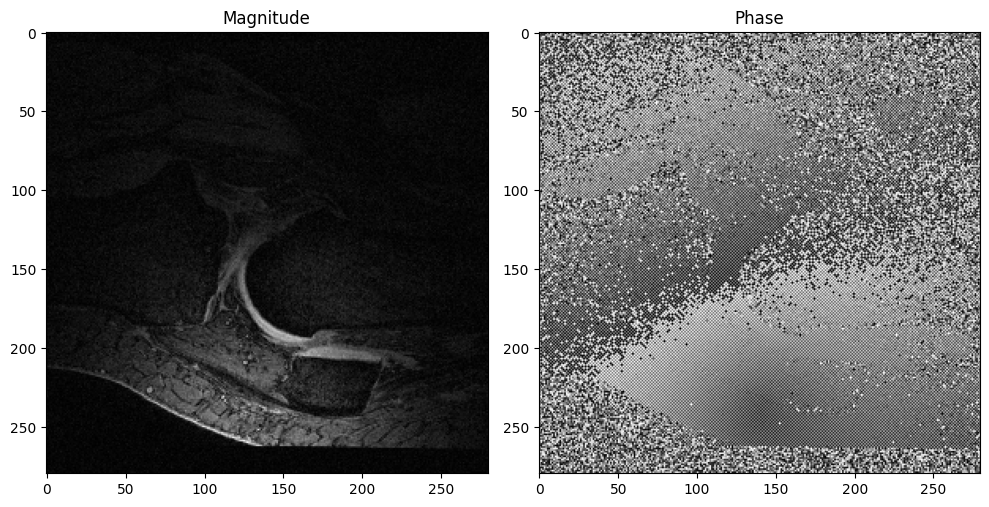
\includegraphics[width=\linewidth]{development_notebook_files/development_notebook_21_0.png}
  \caption{Magnitude and phase image from one coil after inverse FFT (generated in \texttt{notebooks/development.ipynb}).}
\end{figure}

\begin{figure}[p]
  \centering
  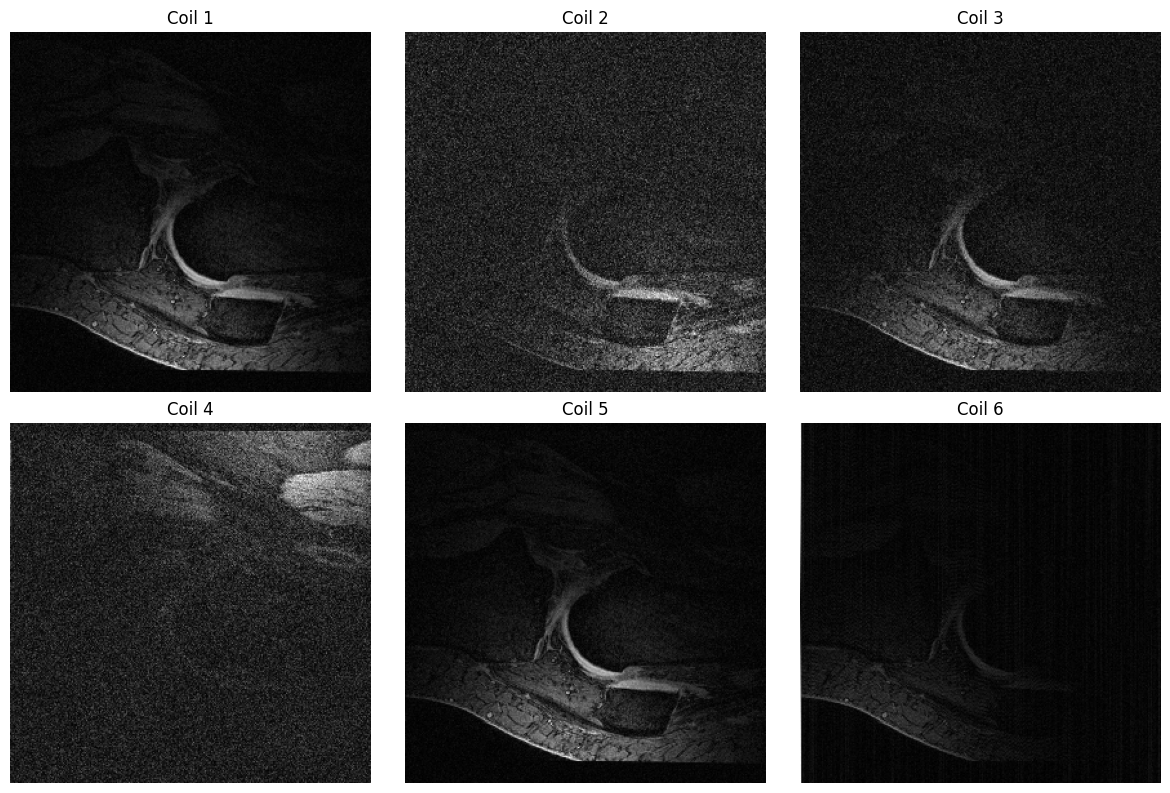
\includegraphics[width=\linewidth]{development_notebook_files/development_notebook_23_0.png}
  \caption{Magnitude images in image space across all coils (generated in \texttt{notebooks/development.ipynb}).}
\end{figure}

\subsubsection*{Coil combination}
Coils were combined using root-sum-of-squares (RSS), \( \sqrt{\sum_c |I_c|^2} \), producing a single magnitude image with improved SNR compared to single-coil images.

\begin{figure}[p]
  \centering
  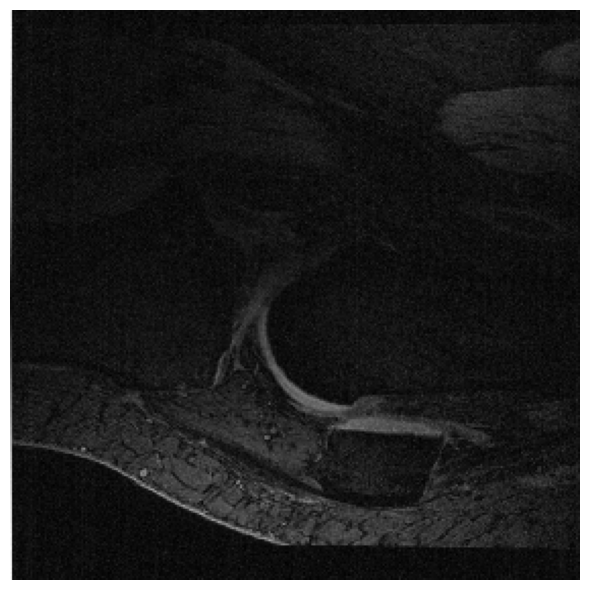
\includegraphics[width=0.75\linewidth]{development_notebook_files/development_notebook_25_0.png}
  \caption{RSS combined magnitude image (generated in \texttt{notebooks/development.ipynb}).}
\end{figure}

\subsection{Exercise 2.2: Removing noise}
\subsubsection*{Three image-space denoisers}
Three denoising methods were applied coil-wise in image space (on magnitude images): Gaussian filtering, bilateral filtering, and wavelet denoising.

\begin{figure}[p]
  \centering
  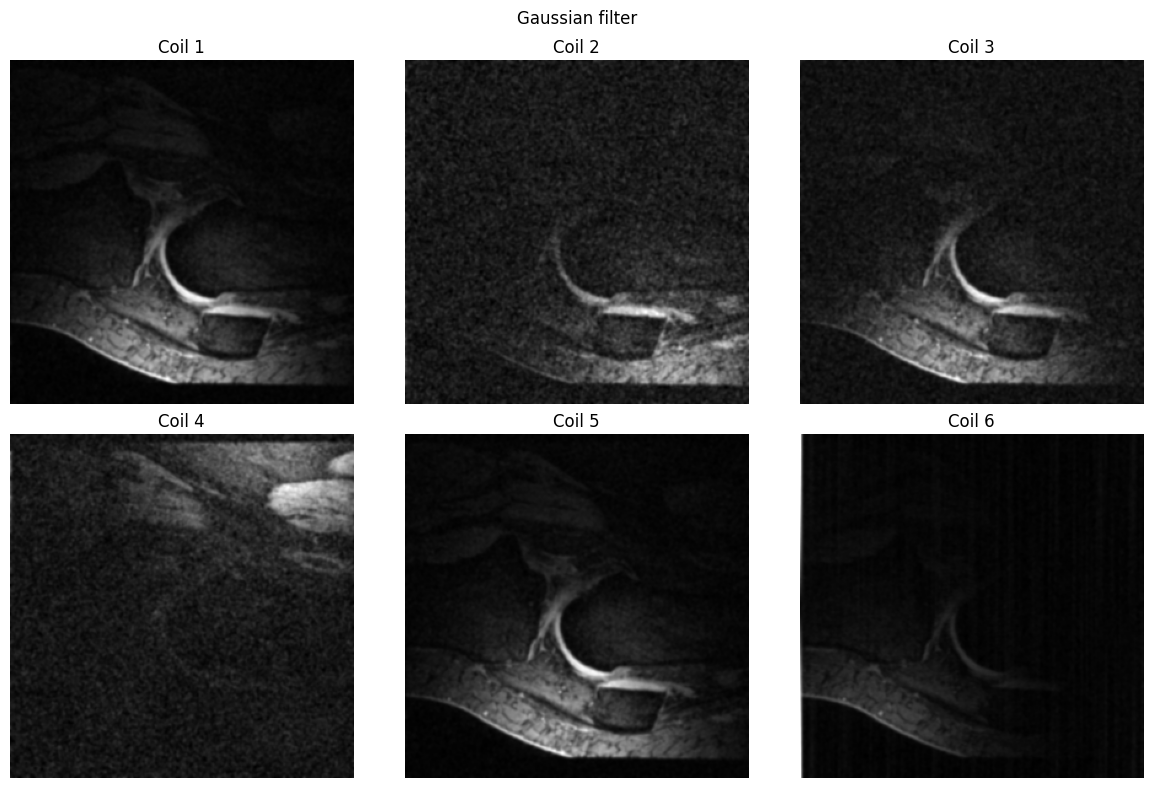
\includegraphics[width=\linewidth]{development_notebook_files/development_notebook_27_0.png}
  \caption{Gaussian denoising applied per coil (generated in \texttt{notebooks/development.ipynb}).}
\end{figure}
\begin{figure}[p]
  \centering
  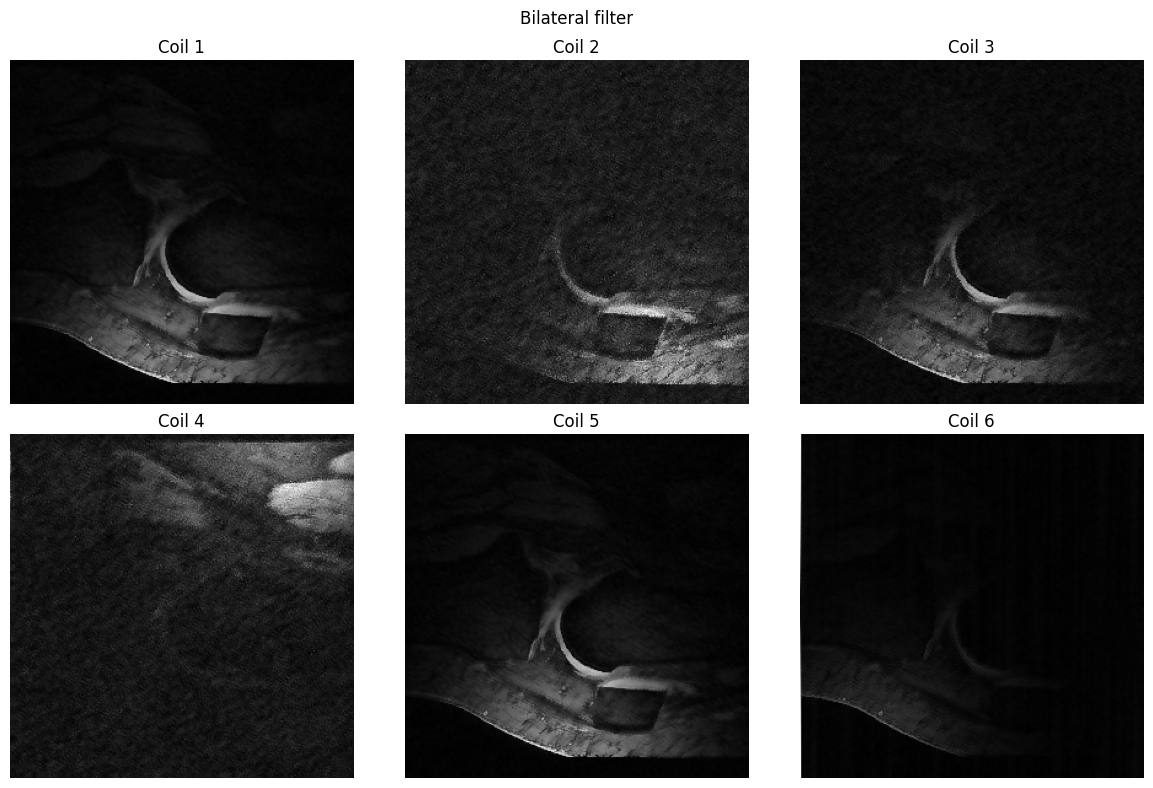
\includegraphics[width=\linewidth]{development_notebook_files/development_notebook_27_1.png}
  \caption{Bilateral denoising applied per coil (generated in \texttt{notebooks/development.ipynb}).}
\end{figure}
\begin{figure}[p]
  \centering
  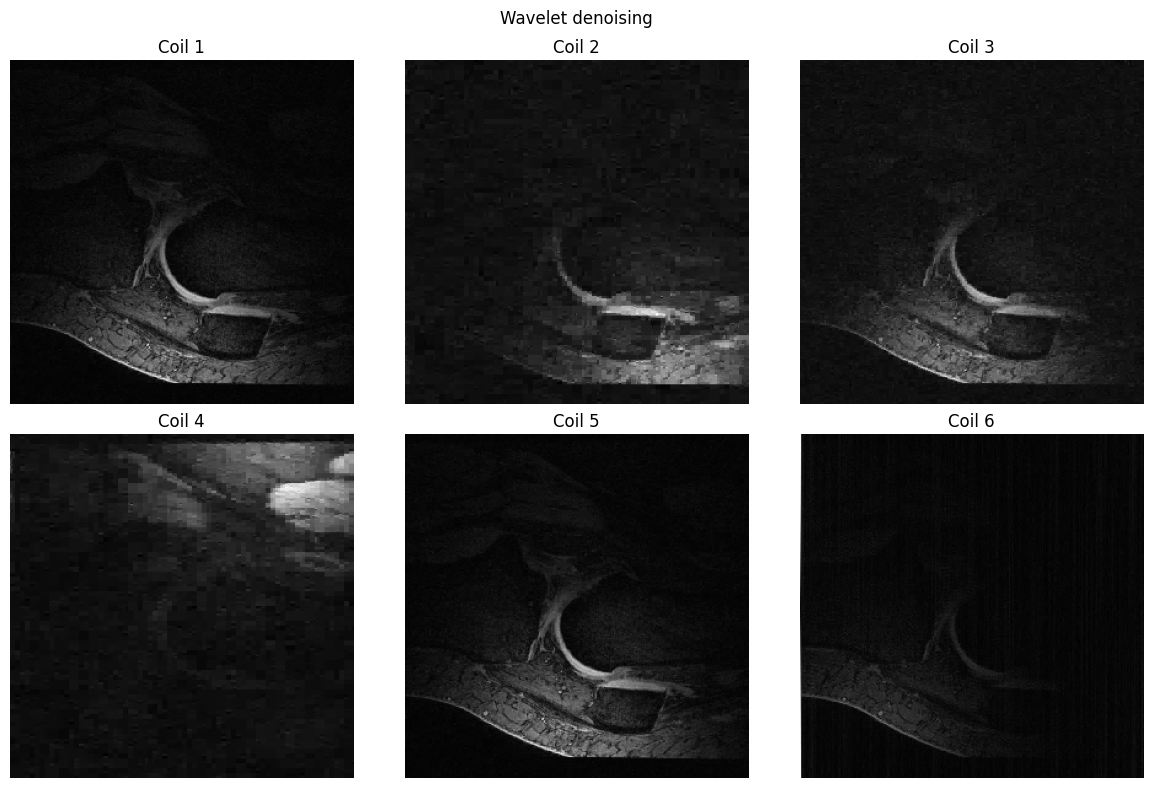
\includegraphics[width=\linewidth]{development_notebook_files/development_notebook_27_2.png}
  \caption{Wavelet denoising applied per coil (generated in \texttt{notebooks/development.ipynb}).}
\end{figure}

\noindent Brief comments (matching the development notebook):
\begin{itemize}
  \item Gaussian: smooths uniformly; reduces noise but blurs edges.
  \item Bilateral: more edge-preserving; smoother flat regions while keeping sharper boundaries.
  \item Wavelet: removes noise-like coefficients across scales; can preserve edges but depends on thresholding.
\end{itemize}

\subsubsection*{k-space Butterworth low-pass}
A Butterworth low-pass filter was applied directly in k-space for the first coil before inverse FFT. This reduces high-frequency noise, but if the cutoff is too aggressive it can blur detail and may introduce ringing.

\begin{figure}[p]
  \centering
  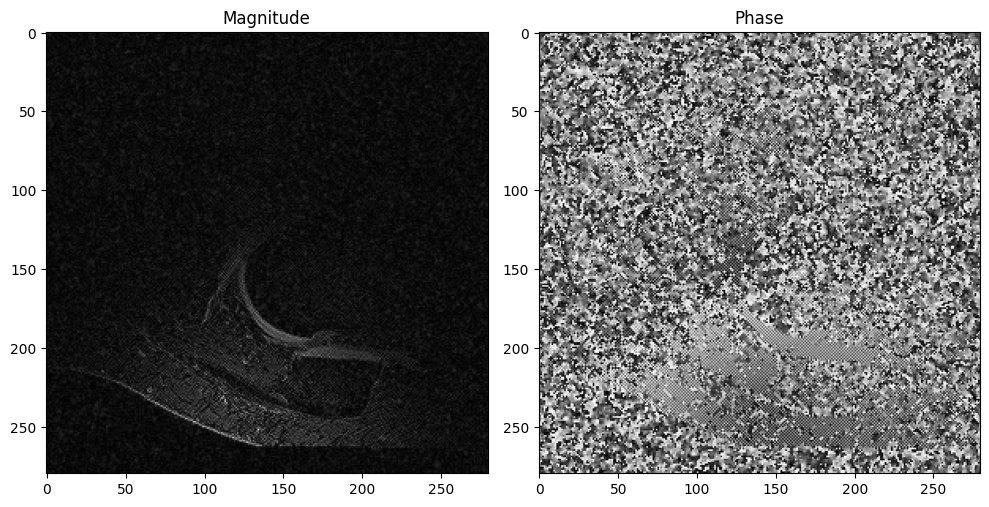
\includegraphics[width=\linewidth]{development_notebook_files/development_notebook_30_0.png}
  \caption{First-coil magnitude and phase after Butterworth low-pass in k-space (generated in \texttt{notebooks/development.ipynb}).}
\end{figure}

\subsubsection*{Denoising on combined image}
Finally, a mild Gaussian filter was applied to the RSS combined image as a simple post-processing step. Stronger filtering would reduce noise further but blur edges.

\begin{figure}[p]
  \centering
  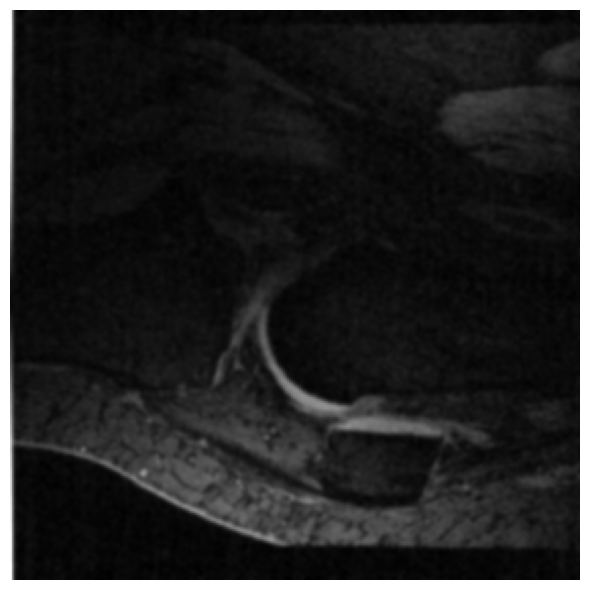
\includegraphics[width=0.75\linewidth]{development_notebook_files/development_notebook_31_0.png}
  \caption{Gaussian denoising applied to the RSS combined image (generated in \texttt{notebooks/development.ipynb}).}
\end{figure}

\section{Module 3: Image segmentation methods (written component)}
\textbf{Note:} The substantive written content for this module must be authored without generative AI assistance. The structure below is provided as a template only.

\subsection{Paper A (processing-based / non-ML)}
% TODO: Bibliographic details (authors, title, venue, year) and a <=10 line summary of what was done.

\subsection{Paper B (ML/DL)}
% TODO: Bibliographic details (authors, title, venue, year) and a <=10 line summary of what was done.

\subsection{Critical comparison (max one page)}
% TODO: Compare scenarios where each works better/worse; advantages, disadvantages, limitations; be specific to the two papers.

\subsection{Proposed improvement (max half page)}
% TODO: Propose one improvement methodology for one selected paper; keep it concrete and testable.

\section*{References}
\begin{thebibliography}{9}
% TODO: Add full, checkable citations here (or switch to a .bib workflow if preferred).
\end{thebibliography}

\appendix
\section{Optional: Included supporting PDFs}
% If you have pre-rendered supplementary material you want appended, place it in report/ and include it like this:
% \includepdf[pages=-]{supplement.pdf}

\end{document}

